\documentclass{standalone}
\usepackage{tikz}
\usetikzlibrary{patterns, positioning}
\usepackage[sfdefault]{ClearSans} %% option 'sfdefault' activates Clear Sans as the default text font
\usepackage[T1]{fontenc}

\begin{document}
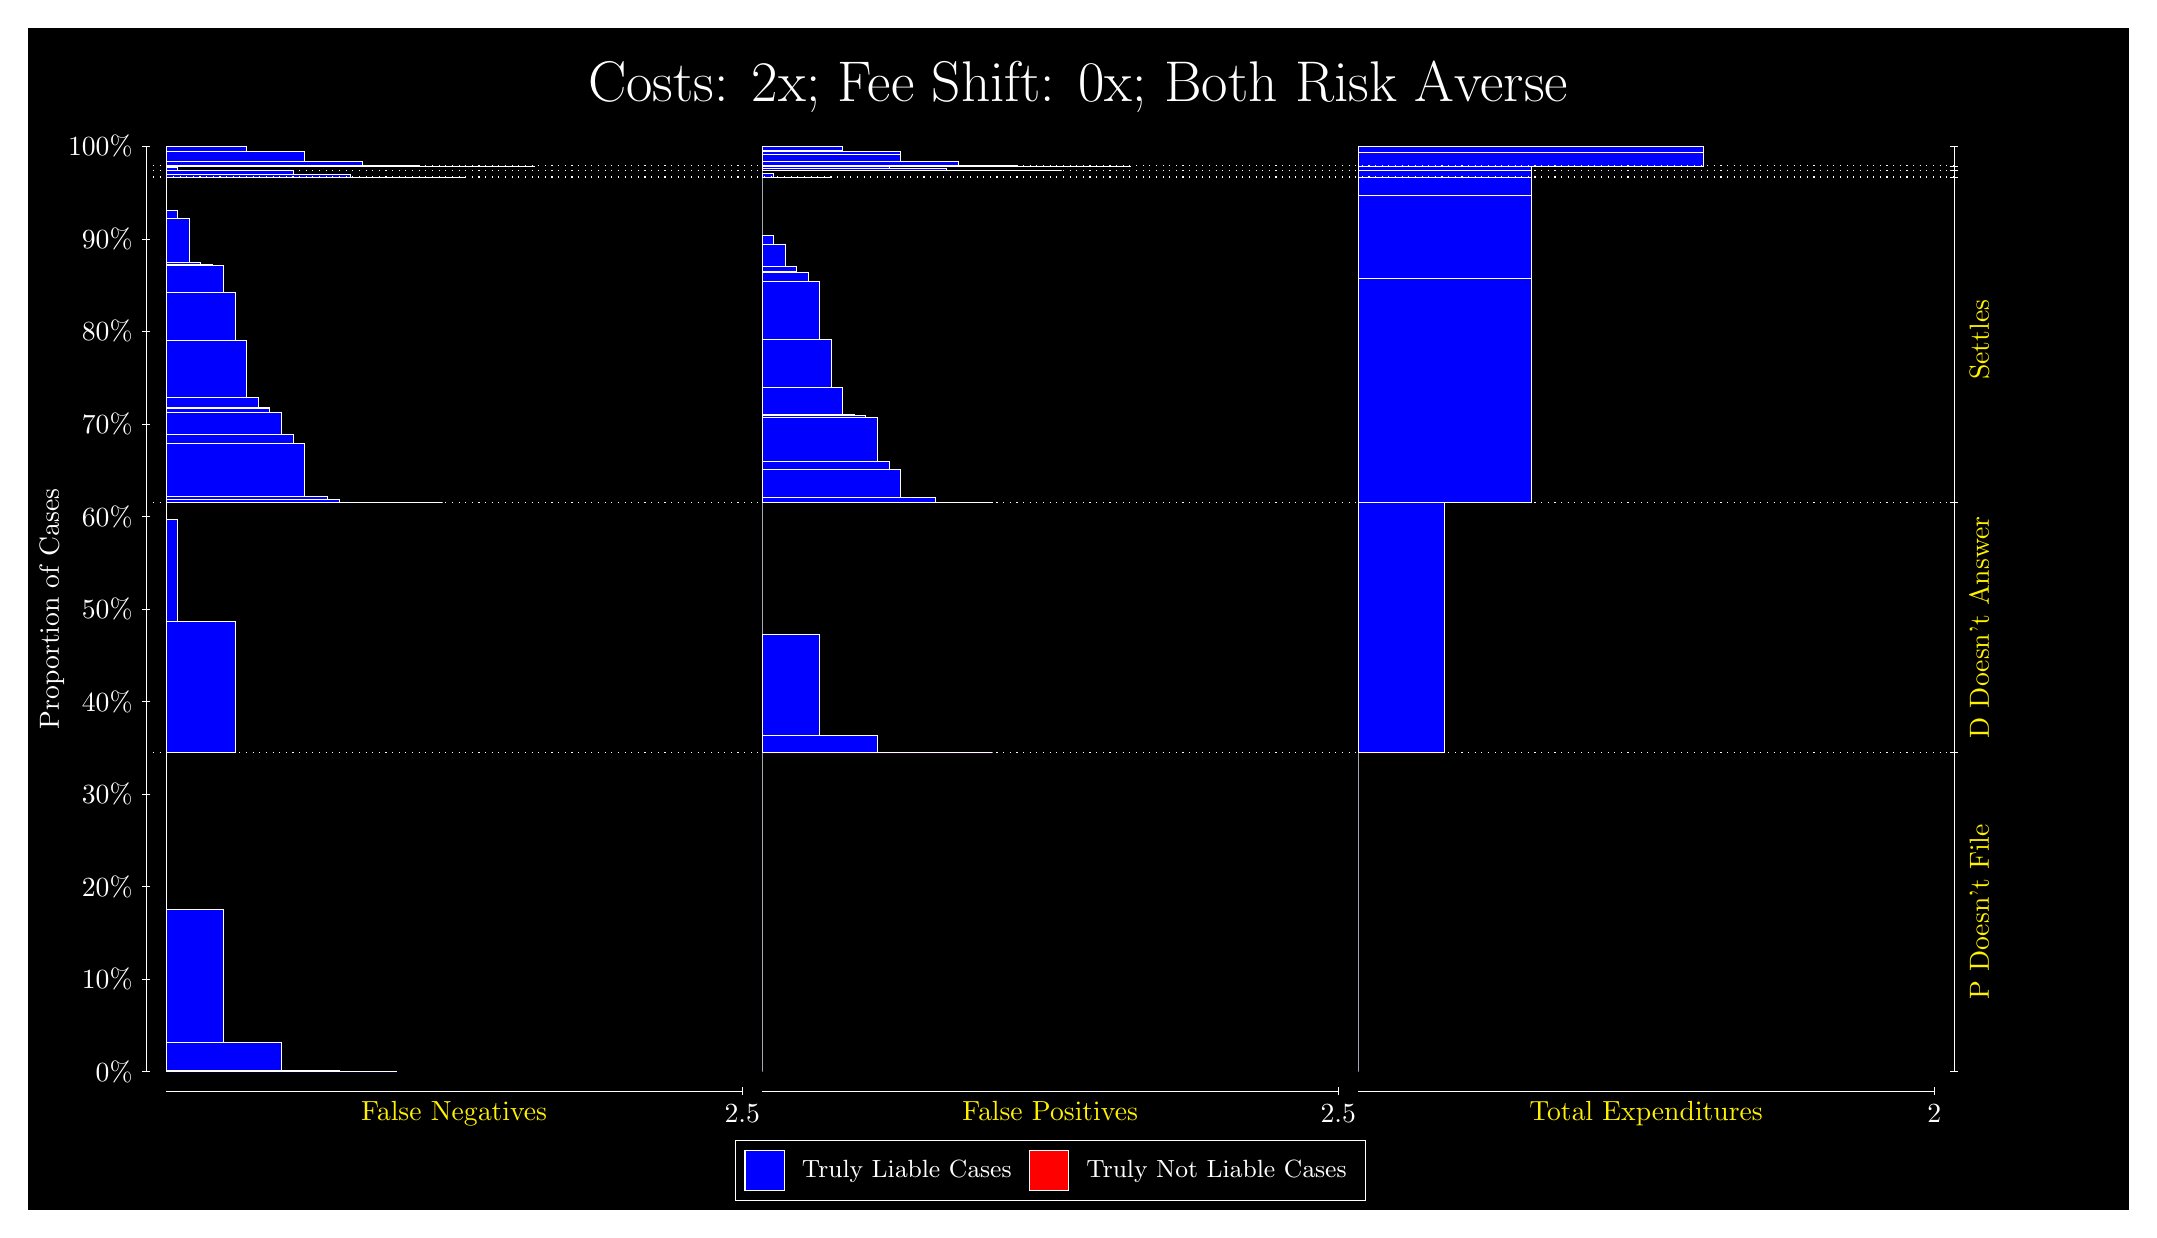
\begin{tikzpicture}
\draw[fill=black] (0,0) rectangle (26.667,15);
\draw[text=white] (0,13.5) rectangle (26.667,15) node[midway] {\huge Costs: 2x; Fee Shift: 0x; Both Risk Averse};
\draw[white, very thin] (1.5,1.75) -- (1.5,13.5);
\node[rotate=90, text=white, anchor=center] at (0.3, 7.625) {Proportion of Cases};
\draw[white, very thin] (1.45,1.75) -- (1.55,1.75);
\node[text=white, anchor=east] at (1.45, 1.75) {0\%};
\draw[white, very thin] (1.45,2.925) -- (1.55,2.925);
\node[text=white, anchor=east] at (1.45, 2.925) {10\%};
\draw[white, very thin] (1.45,4.1) -- (1.55,4.1);
\node[text=white, anchor=east] at (1.45, 4.1) {20\%};
\draw[white, very thin] (1.45,5.275) -- (1.55,5.275);
\node[text=white, anchor=east] at (1.45, 5.275) {30\%};
\draw[white, very thin] (1.45,6.45) -- (1.55,6.45);
\node[text=white, anchor=east] at (1.45, 6.45) {40\%};
\draw[white, very thin] (1.45,7.625) -- (1.55,7.625);
\node[text=white, anchor=east] at (1.45, 7.625) {50\%};
\draw[white, very thin] (1.45,8.8) -- (1.55,8.8);
\node[text=white, anchor=east] at (1.45, 8.8) {60\%};
\draw[white, very thin] (1.45,9.975) -- (1.55,9.975);
\node[text=white, anchor=east] at (1.45, 9.975) {70\%};
\draw[white, very thin] (1.45,11.15) -- (1.55,11.15);
\node[text=white, anchor=east] at (1.45, 11.15) {80\%};
\draw[white, very thin] (1.45,12.325) -- (1.55,12.325);
\node[text=white, anchor=east] at (1.45, 12.325) {90\%};
\draw[white, very thin] (1.45,13.5) -- (1.55,13.5);
\node[text=white, anchor=east] at (1.45, 13.5) {100\%};

\draw[white, very thin] (24.457,1.75) -- (24.457,13.5);
\draw[white, very thin] (24.407,1.75) -- (24.507,1.75);
\node[anchor=west] at (24.407, 1.75) {};
\draw[white, very thin] (24.407,5.8016) -- (24.507,5.8016);
\node[anchor=west] at (24.407, 5.8016) {};
\draw[white, very thin] (24.407,8.9776) -- (24.507,8.9776);
\node[anchor=west] at (24.407, 8.9776) {};
\draw[white, very thin] (24.407,13.111) -- (24.507,13.111);
\node[anchor=west] at (24.407, 13.111) {};
\draw[white, very thin] (24.407,13.195) -- (24.507,13.195);
\node[anchor=west] at (24.407, 13.195) {};
\draw[white, very thin] (24.407,13.251) -- (24.507,13.251);
\node[anchor=west] at (24.407, 13.251) {};
\draw[white, very thin] (24.407,13.5) -- (24.507,13.5);
\node[anchor=west] at (24.407, 13.5) {};

\draw[white, very thin, fill=blue] (1.75,1.75) rectangle (4.6775,1.7501);
\draw[white, very thin, fill=blue] (1.75,1.7501) rectangle (3.9457,1.7618);
\draw[white, very thin, fill=blue] (1.75,1.7618) rectangle (3.2138,2.118);
\draw[white, very thin, fill=blue] (1.75,2.118) rectangle (2.4819,3.8072);
\draw[white, very thin, fill=red] (1.75,3.8072) rectangle (1.75,3.8072);
\draw[white, very thin, fill=blue] (1.75,3.8072) rectangle (1.75,5.8016);
\draw[white, very thin, fill=blue] (1.75,5.8016) rectangle (2.6283,7.4699);
\draw[white, very thin, fill=blue] (1.75,7.4699) rectangle (1.8964,8.7637);
\draw[white, very thin, fill=red] (1.75,8.7637) rectangle (1.75,8.7637);
\draw[white, very thin, fill=blue] (1.75,8.7637) rectangle (1.75,8.9776);
\draw[white, very thin, fill=blue] (1.75,8.9776) rectangle (5.2631,8.9776);
\draw[white, very thin, fill=blue] (1.75,8.9776) rectangle (4.6775,8.9777);
\draw[white, very thin, fill=blue] (1.75,8.9777) rectangle (4.5312,8.9787);
\draw[white, very thin, fill=blue] (1.75,8.9787) rectangle (4.3848,8.9787);
\draw[white, very thin, fill=blue] (1.75,8.9787) rectangle (4.092,8.9791);
\draw[white, very thin, fill=blue] (1.75,8.9791) rectangle (3.9457,9.0132);
\draw[white, very thin, fill=blue] (1.75,9.0132) rectangle (3.7993,9.054);
\draw[white, very thin, fill=blue] (1.75,9.054) rectangle (3.6529,9.0599);
\draw[white, very thin, fill=blue] (1.75,9.0599) rectangle (3.5065,9.7242);
\draw[white, very thin, fill=blue] (1.75,9.7242) rectangle (3.3602,9.8386);
\draw[white, very thin, fill=blue] (1.75,9.8386) rectangle (3.2138,10.117);
\draw[white, very thin, fill=blue] (1.75,10.117) rectangle (3.0674,10.177);
\draw[white, very thin, fill=blue] (1.75,10.177) rectangle (3.0674,10.186);
\draw[white, very thin, fill=blue] (1.75,10.186) rectangle (2.921,10.308);
\draw[white, very thin, fill=blue] (1.75,10.308) rectangle (2.7746,11.038);
\draw[white, very thin, fill=blue] (1.75,11.038) rectangle (2.6283,11.646);
\draw[white, very thin, fill=blue] (1.75,11.646) rectangle (2.4819,11.991);
\draw[white, very thin, fill=blue] (1.75,11.991) rectangle (2.3355,12.006);
\draw[white, very thin, fill=blue] (1.75,12.006) rectangle (2.3355,12.006);
\draw[white, very thin, fill=blue] (1.75,12.006) rectangle (2.1891,12.028);
\draw[white, very thin, fill=blue] (1.75,12.028) rectangle (2.0428,12.592);
\draw[white, very thin, fill=blue] (1.75,12.592) rectangle (1.8964,12.69);
\draw[white, very thin, fill=red] (1.75,12.69) rectangle (1.75,12.69);
\draw[white, very thin, fill=blue] (1.75,12.69) rectangle (1.75,13.111);
\draw[white, very thin, fill=blue] (1.75,13.111) rectangle (5.5558,13.111);
\draw[white, very thin, fill=blue] (1.75,13.111) rectangle (4.8239,13.111);
\draw[white, very thin, fill=blue] (1.75,13.111) rectangle (4.092,13.142);
\draw[white, very thin, fill=blue] (1.75,13.142) rectangle (3.3602,13.194);
\draw[white, very thin, fill=blue] (1.75,13.194) rectangle (2.6283,13.195);
\draw[white, very thin, fill=red] (1.75,13.195) rectangle (1.75,13.195);
\draw[white, very thin, fill=blue] (1.75,13.195) rectangle (2.6283,13.196);
\draw[white, very thin, fill=blue] (1.75,13.196) rectangle (1.8964,13.23);
\draw[white, very thin, fill=red] (1.75,13.23) rectangle (1.75,13.23);
\draw[white, very thin, fill=blue] (1.75,13.23) rectangle (1.75,13.251);
\draw[white, very thin, fill=blue] (1.75,13.251) rectangle (6.4341,13.251);
\draw[white, very thin, fill=blue] (1.75,13.251) rectangle (5.7022,13.251);
\draw[white, very thin, fill=blue] (1.75,13.251) rectangle (4.9703,13.255);
\draw[white, very thin, fill=blue] (1.75,13.255) rectangle (4.2384,13.313);
\draw[white, very thin, fill=blue] (1.75,13.313) rectangle (3.5065,13.438);
\draw[white, very thin, fill=blue] (1.75,13.438) rectangle (2.7746,13.496);
\draw[white, very thin, fill=blue] (1.75,13.496) rectangle (2.0428,13.5);
\draw[white, very thin, fill=red] (1.75,13.5) rectangle (1.75,13.5);
\draw[white, very thin, fill=blue] (1.75,13.5) rectangle (1.75,13.5);
\draw[white, very thin, fill=red] (9.3189,1.75) rectangle (9.3189,1.75);
\draw[white, very thin, fill=blue] (9.3189,1.75) rectangle (9.3189,5.8016);
\draw[white, very thin, fill=red] (9.3189,5.8016) rectangle (12.246,5.8016);
\draw[white, very thin, fill=blue] (9.3189,5.8016) rectangle (12.246,5.8016);
\draw[white, very thin, fill=blue] (9.3189,5.8016) rectangle (11.515,5.8026);
\draw[white, very thin, fill=blue] (9.3189,5.8026) rectangle (10.783,6.0155);
\draw[white, very thin, fill=blue] (9.3189,6.0155) rectangle (10.051,7.3093);
\draw[white, very thin, fill=blue] (9.3189,7.3093) rectangle (9.3189,8.9776);
\draw[white, very thin, fill=red] (9.3189,8.9776) rectangle (12.246,8.9776);
\draw[white, very thin, fill=blue] (9.3189,8.9776) rectangle (12.246,8.9777);
\draw[white, very thin, fill=red] (9.3189,8.9777) rectangle (11.954,8.9777);
\draw[white, very thin, fill=blue] (9.3189,8.9777) rectangle (11.954,8.9777);
\draw[white, very thin, fill=red] (9.3189,8.9777) rectangle (11.661,8.9777);
\draw[white, very thin, fill=blue] (9.3189,8.9777) rectangle (11.661,8.9781);
\draw[white, very thin, fill=blue] (9.3189,8.9781) rectangle (11.515,9.0463);
\draw[white, very thin, fill=red] (9.3189,9.0463) rectangle (11.368,9.0463);
\draw[white, very thin, fill=blue] (9.3189,9.0463) rectangle (11.368,9.0465);
\draw[white, very thin, fill=blue] (9.3189,9.0465) rectangle (11.222,9.0465);
\draw[white, very thin, fill=red] (9.3189,9.0465) rectangle (11.075,9.0465);
\draw[white, very thin, fill=blue] (9.3189,9.0465) rectangle (11.075,9.3987);
\draw[white, very thin, fill=blue] (9.3189,9.3987) rectangle (10.929,9.4965);
\draw[white, very thin, fill=blue] (9.3189,9.4965) rectangle (10.783,10.061);
\draw[white, very thin, fill=blue] (9.3189,10.061) rectangle (10.636,10.082);
\draw[white, very thin, fill=red] (9.3189,10.082) rectangle (10.49,10.082);
\draw[white, very thin, fill=blue] (9.3189,10.082) rectangle (10.49,10.082);
\draw[white, very thin, fill=blue] (9.3189,10.082) rectangle (10.49,10.097);
\draw[white, very thin, fill=blue] (9.3189,10.097) rectangle (10.344,10.443);
\draw[white, very thin, fill=blue] (9.3189,10.443) rectangle (10.197,11.051);
\draw[white, very thin, fill=blue] (9.3189,11.051) rectangle (10.051,11.78);
\draw[white, very thin, fill=blue] (9.3189,11.78) rectangle (9.9044,11.902);
\draw[white, very thin, fill=blue] (9.3189,11.902) rectangle (9.758,11.911);
\draw[white, very thin, fill=blue] (9.3189,11.911) rectangle (9.758,11.971);
\draw[white, very thin, fill=blue] (9.3189,11.971) rectangle (9.6116,12.25);
\draw[white, very thin, fill=blue] (9.3189,12.25) rectangle (9.4652,12.364);
\draw[white, very thin, fill=blue] (9.3189,12.364) rectangle (9.3189,13.111);
\draw[white, very thin, fill=red] (9.3189,13.111) rectangle (10.197,13.111);
\draw[white, very thin, fill=blue] (9.3189,13.111) rectangle (10.197,13.112);
\draw[white, very thin, fill=blue] (9.3189,13.112) rectangle (9.4652,13.163);
\draw[white, very thin, fill=blue] (9.3189,13.163) rectangle (9.3189,13.195);
\draw[white, very thin, fill=red] (9.3189,13.195) rectangle (13.125,13.195);
\draw[white, very thin, fill=blue] (9.3189,13.195) rectangle (13.125,13.195);
\draw[white, very thin, fill=blue] (9.3189,13.195) rectangle (12.393,13.195);
\draw[white, very thin, fill=blue] (9.3189,13.195) rectangle (11.661,13.216);
\draw[white, very thin, fill=blue] (9.3189,13.216) rectangle (10.929,13.25);
\draw[white, very thin, fill=blue] (9.3189,13.25) rectangle (10.197,13.251);
\draw[white, very thin, fill=red] (9.3189,13.251) rectangle (14.003,13.251);
\draw[white, very thin, fill=blue] (9.3189,13.251) rectangle (14.003,13.251);
\draw[white, very thin, fill=red] (9.3189,13.251) rectangle (13.271,13.251);
\draw[white, very thin, fill=blue] (9.3189,13.251) rectangle (13.271,13.251);
\draw[white, very thin, fill=red] (9.3189,13.251) rectangle (12.539,13.251);
\draw[white, very thin, fill=blue] (9.3189,13.251) rectangle (12.539,13.255);
\draw[white, very thin, fill=blue] (9.3189,13.255) rectangle (11.807,13.312);
\draw[white, very thin, fill=red] (9.3189,13.312) rectangle (11.807,13.312);
\draw[white, very thin, fill=blue] (9.3189,13.312) rectangle (11.807,13.313);
\draw[white, very thin, fill=blue] (9.3189,13.313) rectangle (11.075,13.404);
\draw[white, very thin, fill=red] (9.3189,13.404) rectangle (11.075,13.404);
\draw[white, very thin, fill=blue] (9.3189,13.404) rectangle (11.075,13.438);
\draw[white, very thin, fill=blue] (9.3189,13.438) rectangle (10.344,13.454);
\draw[white, very thin, fill=blue] (9.3189,13.454) rectangle (10.344,13.496);
\draw[white, very thin, fill=blue] (9.3189,13.496) rectangle (9.6116,13.496);
\draw[white, very thin, fill=blue] (9.3189,13.496) rectangle (9.6116,13.5);
\draw[white, very thin, fill=blue] (9.3189,13.5) rectangle (9.3189,13.5);
\draw[white, very thin, fill=red] (16.888,1.75) rectangle (16.888,1.75);
\draw[white, very thin, fill=blue] (16.888,1.75) rectangle (16.888,5.8016);
\draw[white, very thin, fill=red] (16.888,5.8016) rectangle (17.986,5.8016);
\draw[white, very thin, fill=blue] (16.888,5.8016) rectangle (17.986,8.9776);
\draw[white, very thin, fill=red] (16.888,8.9776) rectangle (19.083,8.9776);
\draw[white, very thin, fill=blue] (16.888,8.9776) rectangle (19.083,11.825);
\draw[white, very thin, fill=red] (16.888,11.825) rectangle (19.083,11.825);
\draw[white, very thin, fill=blue] (16.888,11.825) rectangle (19.083,12.872);
\draw[white, very thin, fill=red] (16.888,12.872) rectangle (19.083,12.872);
\draw[white, very thin, fill=blue] (16.888,12.872) rectangle (19.083,13.111);
\draw[white, very thin, fill=red] (16.888,13.111) rectangle (19.083,13.111);
\draw[white, very thin, fill=blue] (16.888,13.111) rectangle (19.083,13.195);
\draw[white, very thin, fill=red] (16.888,13.195) rectangle (19.083,13.195);
\draw[white, very thin, fill=blue] (16.888,13.195) rectangle (19.083,13.251);
\draw[white, very thin, fill=red] (16.888,13.251) rectangle (21.279,13.251);
\draw[white, very thin, fill=blue] (16.888,13.251) rectangle (21.279,13.419);
\draw[white, very thin, fill=red] (16.888,13.419) rectangle (21.279,13.419);
\draw[white, very thin, fill=blue] (16.888,13.419) rectangle (21.279,13.5);
\draw[white, dotted] (1.5,5.8016) -- (24.457,5.8016);
\draw[white, dotted] (1.5,8.9776) -- (24.457,8.9776);
\draw[white, dotted] (1.5,13.111) -- (24.457,13.111);
\draw[white, dotted] (1.5,13.195) -- (24.457,13.195);
\draw[white, dotted] (1.5,13.251) -- (24.457,13.251);
\draw[white, very thin] (1.75,1.5) -- (9.0689,1.5);
\node[text=yellow, anchor=north] at (5.4094, 1.5) {False Negatives};
\draw[white, very thin] (9.0689,1.45) -- (9.0689,1.55);
\node[text=white, anchor=north] at (9.0689, 1.45) {2.5};

\draw[white, very thin] (9.3189,1.5) -- (16.638,1.5);
\node[text=yellow, anchor=north] at (12.978, 1.5) {False Positives};
\draw[white, very thin] (16.638,1.45) -- (16.638,1.55);
\node[text=white, anchor=north] at (16.638, 1.45) {2.5};

\draw[white, very thin] (16.888,1.5) -- (24.207,1.5);
\node[text=yellow, anchor=north] at (20.547, 1.5) {Total Expenditures};
\draw[white, very thin] (24.207,1.45) -- (24.207,1.55);
\node[text=white, anchor=north] at (24.207, 1.45) {2};

\node[text=yellow, centered, rotate=90] at (24.777, 3.7758) {P Doesn't File};
\node[text=yellow, centered, rotate=90] at (24.777, 7.3896) {D Doesn't Answer};
\node[text=yellow, centered, rotate=90] at (24.777, 11.044) {Settles};




\draw (12.978300999999998,1.5) node[draw=none] (baseCoordinate) {};
\begin{scope}[align=center]
        \matrix[scale=0.5, draw=white, below=0.5cm of baseCoordinate, nodes={draw}, column sep=0.1cm]{
            \node[rectangle, draw, minimum width=0.5cm, minimum height=0.5cm, fill=blue] {}; &
            \node[draw=none, font=\small, text=white] (B) {Truly Liable Cases}; &
            \node[rectangle, draw, minimum width=0.5cm, minimum height=0.5cm, fill=red] {}; &
            \node[draw=none, font=\small, text=white] (B) {Truly Not Liable Cases}; \\
            };
\end{scope}

\end{tikzpicture}
\end{document}